%%%%%%%%%%%%%%%%%%%%%%%%%%%%%%%%%%%%%%%%%%%%%%%%%%%%%%%%%%
%%%%%%%%%%%%%%%%%%%%%%%%%%%%%%%%%%%%%%%%%%%%%%%%%%%%%%%%%%
%
%                                        PRE-AMBLE
%
%%%%%%%%%%%%%%%%%%%%%%%%%%%%%%%%%%%%%%%%%%%%%%%%%%%%%%%%%%
%%%%%%%%%%%%%%%%%%%%%%%%%%%%%%%%%%%%%%%%%%%%%%%%%%%%%%%%%%

\documentclass[11pt]{amsart}

%------------------------------------ LOAD PACKAGES ----

\usepackage{amsfonts, amsthm, amssymb, amsmath, stmaryrd, etoolbox}
\usepackage{comment}
\usepackage{mathtools}
\usepackage{graphicx,caption,subcaption}

\usepackage[inline]{enumitem}
\setlist{itemsep=0em, topsep=0em, parsep=0em}
\setlist[enumerate]{label=(\alph*)}
\usepackage{tikz}
\usetikzlibrary{matrix,arrows}


\definecolor{mycolor}{rgb}{0,0,0.7}
\usepackage{hyperref}
\hypersetup{colorlinks,linkcolor={mycolor},citecolor={mycolor},urlcolor={mycolor}}

%------------------------------------ NEW COMMANDS ------

\newcommand{\RR}{\mathbb{R}}
\newcommand{\ZZ}{\mathbb{Z}}
\newcommand{\NN}{\mathbb{N}}
\newcommand{\QQ}{\mathbb{Q}}
\newcommand{\CC}{\mathbb{C}}
\renewcommand{\epsilon}{\varepsilon}

\newcommand{\cl}[1]{\mathcal{#1}}
\newcommand{\scr}[1]{\mathscr{#1}}
\newcommand{\op}[1]{\operatorname{#1}}
\newcommand{\cat}[1]{\mathbf{#1}}
\renewcommand{\t}[1]{\textup{#1}}

\newcommand{\from}{\colon}
\newcommand{\xto}[1]{\xrightarrow{#1}}
\newcommand{\sm}{\smallsetminus}
\renewcommand{\span}{\xrightarrow{\mathit{sp}}}
\newcommand{\cospan}{\xrightarrow{\mathit{csp}}}
\renewcommand{\ss}[2]{_{#1}^{#2}}

\newcommand{\csC}{\widetilde{\mathbf{C}}}

\newcommand{\diagram}[1]{\raisebox{-0.5\height}{\includegraphics{#1}}}

%---------------------------- DECLARE MATH OPERATORS ----

\DeclareMathOperator{\Hom}{Hom}
\DeclareMathOperator{\id}{id}
\DeclareMathOperator{\ob}{Ob}
\DeclareMathOperator{\arr}{arr}
\DeclareMathOperator{\im}{im}
\DeclareMathOperator{\Aut}{Aut}
\DeclareMathOperator{\Bij}{Bij}
\DeclareMathOperator{\Sub}{Sub}

%------------------------- ENVIRONMENTS AND COUNTERS-----

\newtheorem{thm}{Theorem}[section]
\newtheorem{lem}[thm]{Lemma}
\newtheorem{prop}[thm]{Proposition}
\newtheorem{cor}[thm]{Corollary}

\theoremstyle{remark}
\newtheorem{remark}[thm]{Remark}
\newtheorem{notation}[thm]{Notation}

\theoremstyle{definition}
\newtheorem{ex}[thm]{Example} 
\newtheorem{defn}[thm]{Definition}

\setcounter{tocdepth}{1} % Sets depth for table of contents. 

%%%%%%%%%%%%%%%%%%%%%%%%%%%%%%%%%%%%%%%%%%%%%%%%%%%%%%%%%
%%%%%%%%%%%%%%%%%%%%%%%%%%%%%%%%%%%%%%%%%%%%%%%%%%%%%%%%%
%%%%%%%%%%%%%%%%%%%%%%%%%%%%%%%%%%%%%%%%%%%%%%%%%%%%%%%%%
%%%%%%%%%%%%%%%%%%%%%%%%%%%%%%%%%%%%%%%%%%%%%%%%%%%%%%%%%
%
%                                    BEGIN DOCUMENT
%
%%%%%%%%%%%%%%%%%%%%%%%%%%%%%%%%%%%%%%%%%%%%%%%%%%%%%%%%%
%%%%%%%%%%%%%%%%%%%%%%%%%%%%%%%%%%%%%%%%%%%%%%%%%%%%%%%%%
%%%%%%%%%%%%%%%%%%%%%%%%%%%%%%%%%%%%%%%%%%%%%%%%%%%%%%%%%
%%%%%%%%%%%%%%%%%%%%%%%%%%%%%%%%%%%%%%%%%%%%%%%%%%%%%%%%%

\begin{document}
	

%%%%%%%%%%%%%%%%%%%%%%%%%%%%%%%%%%%%%%%%%%%%%%%%%%%%%%%%%%
%
\section{Cooking up a fibration} %                   INTRODUCTION
\label{sec.Cooking}
%
%%%%%%%%%%%%%%%%%%%%%%%%%%%%%%%%%%%%%%%%%%%%%%%%%%%%%%%%%%
Let $\cat{S}$ be a skeleton of the groupoid of finite sets and bijections.  Define a functor $F \from \cat{S} \to \cat{S}$ by $X \mapsto X + \{X\}$ on objects and $\sigma \mapsto \sigma + \id_{\{X\}}$.  We will construct a groupoid $\cat{S}'$ equivalent to $\cat{S}$ and a fibration $F' \from \cat{S}' \to \cat{S}'$ such that
\begin{equation}
\label{eq:sub F' for F}
\raisebox{-0.75\height}{
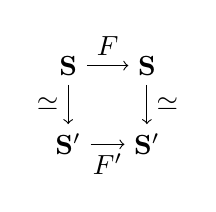
\begin{tikzpicture}
	\node (1) at (-0.5,1) {$\cat{S}$};
	\node (2) at (-0.5,0) {$\cat{S}'$};
	\node (3) at (0.5,0) {$\cat{S}'$};
	\node (4) at (0.5,1) {$\cat{S}$};
	%
	\draw [->] (1) to node[left] {$\simeq$} (2);
	\draw [->] (2) to node[below] {$F'$} (3);
	\draw [->] (1) to node[above] {$F$} (4);
	\draw [->] (4) to node[right] {$\simeq$} (3);
\end{tikzpicture} 
}
\end{equation}

Construct a category $\cat{S}'$ with
\begin{itemize}
	\item (objects) pairs $(\mathbf{m},f)$ where $\mathbf{m}=\{0,1,\dotsc,m-1\}$ and $f \from \NN \setminus \mathbf{m} \to \NN$ is any set injection, and
	\item (arrows) $\cat{S}'((\mathbf{m},f),(\mathbf{n},g))$ is empty if $m \neq n$, else consists of bijections $\alpha \from \NN \to \NN$ such that
	\[
	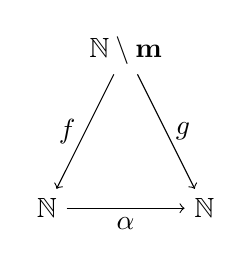
\begin{tikzpicture}
		\node (1) at (0,2) {$\NN \setminus \mathbf{m}$};
		\node (2) at (-1,0) {$\NN$};
		\node (3) at (1,0) {$\NN$};
		%
		\draw [->] (1) to node[left] {$f$} (2);
		\draw [->] (1) to node[right] {$g$} (3);
		\draw [->] (2) to node[below] {$\alpha$} (3);
	\end{tikzpicture}
	\]
\end{itemize}

\begin{lem}
	There is an equivalence of categories $\cat{S} \simeq \cat{S}'$ via the functor 
	\[
		e \from \cat{S} \to \cat{S}'
	\] 
	defined by 
	\begin{itemize}
		\item (objects) $e(\mathbf{m}) = (\mathbf{m},\iota)$ with $\iota \from \NN \setminus \mathbf{m} \hookrightarrow \NN$ is the inclusion, and
		\item (arrows) $e(\sigma) \from (\mathbf{m},\iota) \to (\mathbf{m},\iota)$ is the bijection $\sigma + \id \from \NN \to \NN$ that acts by $\sigma$ on $\mathbf{m}$ and the identity on $\NN \setminus \mathbf{m}$.
	\end{itemize}
\end{lem}

\begin{proof}
	We start with the claim that two objects $(\mathbf{m},f)$ and $(\mathbf{n},g)$ in $\cat{S}'$ are isomorphic if and only if $m=n$.  Essential surjectivity follows from this claim since, for every natural number $k$, there is the element $(\mathbf{k}, \iota)$ in the image of $e$.
	
	The sufficiency of the claim is obvious since there are no arrows to establish an isomorphism if $m \neq n$.  Conversely, define a map $\alpha \from \NN \to \NN$ to be any bijection such that $\alpha (f(k))=g(k)$ for $k \in \NN \setminus \mathbf{m}$. The latter requirement ensures that 
	\[
	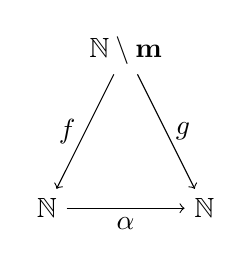
\begin{tikzpicture}
		\node (1) at (0,2) {$\NN \setminus \mathbf{m}$};
		\node (2) at (-1,0) {$\NN$};
		\node (3) at (1,0) {$\NN$};
		%
		\draw [->] (1) to node[left] {$f$} (2);
		\draw [->] (1) to node[right] {$g$} (3);
		\draw [->] (2) to node[below] {$\alpha$} (3);
	\end{tikzpicture}
	\]
	commutes. This proves the claim and, therefore, the essential surjectivity of $e$.
	
	Note that $\cat{S'}((\mathbf{m},\iota),(\mathbf{m},\iota))$ consists of exactly the bijections $\NN \to \NN$ that fix $k$ when $k \in \NN \setminus \mathbf{m}$.  But this is exactly the permutations on $\mathbf{m}$. The fullness and faithfulness of $e$ follow.  
\end{proof}

The next step is to construct our fibration. Define a functor $F' \from \cat{S}' \to \cat{S}'$ as follows:
\begin{itemize}
	\item (objects) $F' (\mathbf{m},f) = (\mathbf{m+1},f|_{\NN \setminus \mathbf{m+1}})$, and 
	\item (arrows) given any map
	\[
	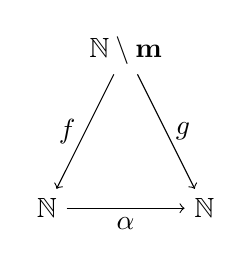
\begin{tikzpicture}
		\node (1) at (0,2) {$\NN \setminus \mathbf{m}$};
		\node (2) at (-1,0) {$\NN$};
		\node (3) at (1,0) {$\NN$};
		%
		\draw [->] (1) to node[left] {$f$} (2);
		\draw [->] (1) to node[right] {$g$} (3);
		\draw [->] (2) to node[below] {$\alpha$} (3);
	\end{tikzpicture}
	\]
	define $F'(\alpha) \from (\mathbf{m},f|_{\NN \setminus \mathbf{m+1}}) \to (\mathbf{m},g|_{\NN \setminus \mathbf{m+1}})$ to be given by
	\[
	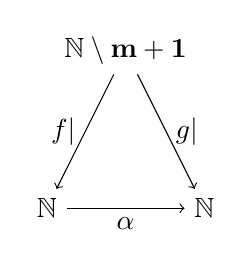
\begin{tikzpicture}
		\node (1) at (0,2) {$\NN \setminus \mathbf{m+1}$};
		\node (2) at (-1,0) {$\NN$};
		\node (3) at (1,0) {$\NN$};
		%
		\draw [->] (1) to node[left] {$f|$} (2);
		\draw [->] (1) to node[right] {$g|$} (3);
		\draw [->] (2) to node[below] {$\alpha$} (3);
	\end{tikzpicture}
	\]
\end{itemize}

\begin{lem}
	The functor $F'$ is a fibration.
\end{lem}
\begin{proof}
	Suppose $F'(\mathbf{m},f)=(\mathbf{m+1},f|_{\NN \setminus \mathbf{m+1}})$ and we have an arrow
	\[
	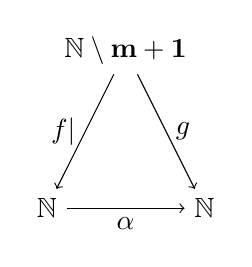
\begin{tikzpicture}
		\node (1) at (0,2) {$\NN \setminus \mathbf{m+1}$};
		\node (2) at (-1,0) {$\NN$};
		\node (3) at (1,0) {$\NN$};
		%
		\draw [->] (1) to node[left] {$f|$} (2);
		\draw [->] (1) to node[right] {$g$} (3);
		\draw [->] (2) to node[below] {$\alpha$} (3);
	\end{tikzpicture}
	\]
Then this arrow is in the image of 
	\[
	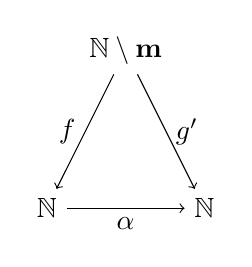
\begin{tikzpicture}
		\node (1) at (0,2) {$\NN \setminus \mathbf{m}$};
		\node (2) at (-1,0) {$\NN$};
		\node (3) at (1,0) {$\NN$};
		%
		\draw [->] (1) to node[left] {$f$} (2);
		\draw [->] (1) to node[right] {$g'$} (3);
		\draw [->] (2) to node[below] {$\alpha$} (3);
	\end{tikzpicture}
	\]
where $g' = \alpha f$.  Indeed, $g'|_{\NN \setminus \mathbf{m+1}} = (\alpha f)|_{\NN \setminus \mathbf{m+1}} = \alpha (f|_{\NN \setminus \mathbf{m+1}}) = g$.  
\end{proof}

For what it's worth, $F'$ is faithful and this is easy to show.  It is not full, since $\cat{S}'$ is equivalent to $\cat{S}$ and so for each $m$, there are $m!$ maps between $(\mathbf{m},f)$ and $(\mathbf{m+1},g)$ for any $f$ and $g$, but there are $(m+1)!$ maps between $F'(\mathbf{m},f)=(\mathbf{m+1},f)$ and $F'(\mathbf{m},g)=(\mathbf{m+1},g)$.  

It remains to show that \eqref{eq:sub F' for F} commutes.  Chasing a set $\mathbf{m}$ around the upper right path of \eqref{eq:sub F' for F}, we land on $(\mathbf{m+1},\iota)$ which is the same if we chase $\mathbf{m}$ around the lower left path.  Chasing a bijection $\sigma \from \mathbf{m} \to \mathbf{m}$ around the upper right path, we land on the arrow
\[
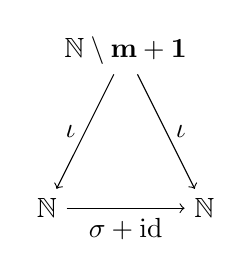
\begin{tikzpicture}
	\node (1) at (0,2) {$\NN \setminus \mathbf{m+1}$};
	\node (2) at (-1,0) {$\NN$};
	\node (3) at (1,0) {$\NN$};
	%
	\draw [->] (1) to node[left] {$\iota$} (2);
	\draw [->] (1) to node[right] {$\iota$} (3);
	\draw [->] (2) to node[below] {$\sigma + \id$} (3);
\end{tikzpicture}
\]
where the $\sigma$ acts on $\mathbf{m}$ and the $\id$ acts on $\NN \setminus \mathbf{m}$.  This is the same if we chase $\sigma$ around the lower left path.

%%%%%%%%%%%%%%%%%%%%%%%%%%%%%%%%%%%%%%%%%%%%%%%%%%%%%%%%%%
%
\section{Computing some pullbacks} %       INTRODUCTION
\label{sec.Computing}
%
%%%%%%%%%%%%%%%%%%%%%%%%%%%%%%%%%%%%%%%%%%%%%%%%%%%%%%%%%%

We are going to try to construct a bicategory with 
\begin{itemize}
	\item (objects) groupoids,
	\item ($1$-morphisms) spans of groupoid fibrations, and
	\item ($2$-morphisms) are spans of spans of groupoid fibrations up to equivalence.
\end{itemize} 
By up to equivalence, we mean that a pair of parallel $2$-morphisms are identified whenever there is an equivalence of groupoids $\theta$ so that 
\[
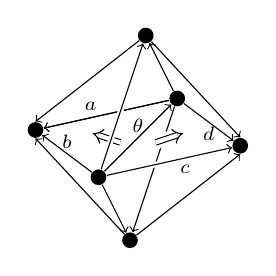
\begin{tikzpicture}
	\node [circle,fill=black,inner sep=2pt] (v1) at (-1.4,-1) {};
	\node [circle,fill=black,inner sep=2pt] (v2) at (-0.2,-2.4) {};
	\node [circle,fill=black,inner sep=2pt] (v3) at (1.2,-1.2) {};
	\node [circle,fill=black,inner sep=2pt] (v4) at (0.4,-0.6) {};
	\node [circle,fill=black,inner sep=2pt] (v5) at (-0.6,-1.6) {};
	\node [circle,fill=black,inner sep=2pt] (v6) at (0,0.2) {};
	\node (v7) at (-0.2,-1.2) {};
	\node (v8) at (-0.8,-1) {};
	\node (v9) at (0,-1.2) {};
	\node (v10) at (0.6,-1) {};
	%
	%
	%
	\draw [->]  (v6) edge (v1.north);
	\draw [->] (v2) edge (v1.south);
	\draw [->] (v4) edge (v1);
	\draw [->] (v4) edge node[shift={(-0.2,0.1)}] {\scriptsize $a$} (v1);
	\draw [->]  (v5) edge node[shift={(0.0,0.15)}] {\scriptsize $b$} (v1);
	\draw [->]  (v5) edge (v2);
	\draw [->]  (v4) edge (v2);
	\draw [->] (v6) edge (v3.north);
	\draw [->]  (v2) edge (v3.south);
	\draw [->]  (v4) edge node[shift={(0.0,-0.15)}] {\scriptsize $d$} (v3);
	\draw [->,line width=2,white]  (v5) edge (v3);
	\draw [->]  (v5) edge node[shift={(0.2,-0.1)}] {\scriptsize $c$} (v3);
	\draw [->] (v5) edge node[shift={(0,0.15)}] {\scriptsize $\theta$} (v4);
	\draw [->] (v4) edge (v6);
	\draw [-implies,double,double equal sign distance] (v7) -- (v8);
	\draw [->,line width=2,white]  (v5) edge (v6);
	\draw [->]  (v5) edge (v6);
	\draw [-,line width=5,white] (v9) -- (v10);
	\draw [-implies,double,double equal sign distance] (v9) -- (v10);
\end{tikzpicture}
\]
the outside faces of the diagram commute and there are natural isomorphisms $b \Rightarrow a \theta$ and $c \Rightarrow d \theta$.

Inside of this bicategory, we pick out two important $1$-morphisms
\[
	A^\dagger \coloneqq 
	\raisebox{-0.5\height}{
	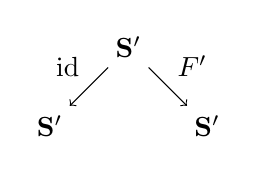
\begin{tikzpicture}
		\node (lleg) at (-1,0) {$\cat{S}'$};
		\node (apex) at (0,1) {$\cat{S}'$};
		\node (rleg) at (1,0) {$\cat{S}'$};
		%
		\draw [->] (apex) to node[above left] {$\id$} (lleg);
		\draw [->] (apex) to node[above right] {$F'$} (rleg);
	\end{tikzpicture}
	}
	\quad \quad 
	A \coloneqq 
	\raisebox{-0.5\height}{
	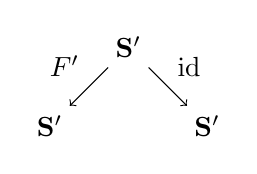
\begin{tikzpicture}
		\node (lleg) at (-1,0) {$\cat{S}'$};
		\node (apex) at (0,1) {$\cat{S}'$};
		\node (rleg) at (1,0) {$\cat{S}'$};
		%
		\draw [->] (apex) to node[above right] {$\id$} (rleg);
		\draw [->] (apex) to node[above left] {$F'$} (lleg);
	\end{tikzpicture}
	}
\]
where $F'$ is the fibration constructed above.

The composition $AA^\dagger$ is the span of groupoids
\[
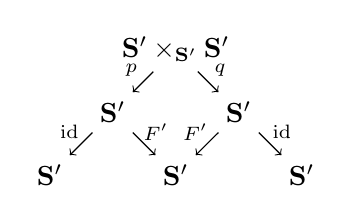
\begin{tikzpicture}
	\node (v1) at (0,0) {$\cat{S'} \times_{\cat{S'}} \cat{S'}$};
	\node (v2) at (-0.8,-0.8) {$\cat{S'}$};
	\node (v3) at (0,-1.6) {$\cat{S'}$};
	\node (v4) at (0.8,-0.8) {$\cat{S'}$};
	\node (v5) at (-1.6,-1.6) {$\cat{S'}$};
	\node (v6) at (1.6,-1.6) {$\cat{S'}$};
	%
	\draw [->]  (v1) edge node [shift={(-0.15,0.15)}] {\scriptsize $p$} (v2);
	\draw [->] (v1) edge node [shift={(0.15,0.15)}] {\scriptsize $q$} (v4);
	\draw [->]  (v2) edge node [shift={(-0.15,0.15)}] {\scriptsize $\id$} (v5);
	\draw [->] (v2) edge node [shift={(0.15,0.15)}] {\scriptsize $F'$} (v3);
	\draw [->]  (v4) edge node [shift={(-0.15,0.15)}] {\scriptsize $F'$} (v3);
	\draw [->]  (v4) edge node [shift={(0.15,0.15)}] {\scriptsize $\id$} (v6);
\end{tikzpicture}
\]
Now because $F'$ is a fibration, which are preserved under pullback, we know that $p$ and $q$ are fibrations too.  The pullback $\cat{S}' \times_{\cat{S}'} \cat{S}'$ is the groupoid with 
\begin{itemize}
	\item (objects) pairs $((\mathbf{m}f),(\mathbf{m},g))$ of objects in $\cat{S}'$ such that the restrictions of $f$ and $g$ to $\NN \setminus \mathbf{m+1}$ coincide,
	\item (arrows) are pairs of morphisms
	\[
	\left(
	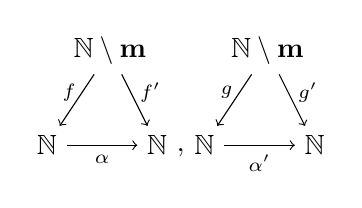
\begin{tikzpicture}[baseline=12mm] 
		\begin{scope}
		\node (v1) at (0,2) {$\mathbb{N} \setminus \mathbf{m}$};
		\node (v2) at (-0.8,0.8) {$\mathbb{N}$};
		\node (v3) at (0.6,0.8) {$\mathbb{N}$};
		%
		\draw [->] (v1) to node[shift={(-0.1,0.1)}] {\scriptsize $f$} (v2);
		\draw [->] (v1) to node[shift={(0.2,0.1)}] {\scriptsize $f'$} (v3);
		\draw [->] (v2) to node[below] {\scriptsize$\alpha$} (v3);
		\end{scope}
		\begin{scope}[shift={(2,0)}]
		\node (v1) at (0,2) {$\mathbb{N} \setminus \mathbf{m}$};
		\node (v2) at (-0.8,0.8) {$\mathbb{N}$};
		\node (v3) at (0.6,0.8) {$\mathbb{N}$};
		%
		\draw [->] (v1) to node [shift={(-0.1,0.1)}] {\scriptsize $g$} (v2);
		\draw [->] (v1) to node [shift={(0.2,0.1)}] {\scriptsize $g'$} (v3);
		\draw [->] (v2) to node [below] {\scriptsize $\alpha'$} (v3);
		\end{scope}
		%
		\node at (0.9,0.7) {,};
	\end{tikzpicture}
	\right)
	\]
	such that $f|_{\NN \setminus \mathbf{m+1}} = g|_{\NN \setminus \mathbf{m+1}}$, $f'|_{\NN \setminus \mathbf{m+1}} = g'|_{\NN \setminus \mathbf{m+1}}$, and $\alpha = \alpha'$.
\end{itemize}

Then a trivial calculation gives us that $A^\dagger A$ is the span
\[
	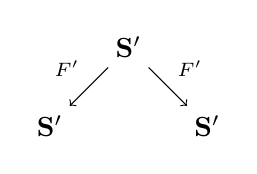
\begin{tikzpicture}
		\node (lleg) at (-1,0) {$\cat{S}'$};
		\node (apex) at (0,1) {$\cat{S}'$};
		\node (rleg) at (1,0) {$\cat{S}'$};
		%
		\draw [->] (apex) to node[above left] {\scriptsize $F'$} (lleg);
		\draw [->] (apex) to node[above right] {\scriptsize $F'$} (rleg);
	\end{tikzpicture}
\]
These spans are really $1$-morphisms in a symmetric monoidal bicategory, and so we can take the coproduct $A^\dagger A + \id_{\cat{S}'}$. This is the span
\[
	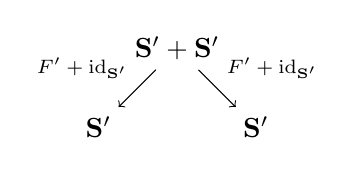
\begin{tikzpicture}
		\node (lleg) at (-1,0) {$\cat{S}'$};
		\node (apex) at (0,1) {$\cat{S}'+\cat{S}'$};
		\node (rleg) at (1,0) {$\cat{S}'$};
		%
		\draw [->] (apex) to node[above left] {\scriptsize $F'+\id_{\cat{S}'}$} (lleg);
		\draw [->] (apex) to node[above right] {\scriptsize $F'+\id_{\cat{S}'}$} (rleg);
	\end{tikzpicture}
\]
The $2$-morphisms is this symmetric monoidal bicategory casually mentioned above are spans of spans in the category of groupoids and fibrations and so we want to find an invertible $2$-morphism of the form
\[
	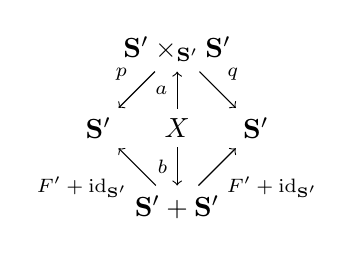
\begin{tikzpicture}
		\node (lleg) at (-1,0) {$\cat{S}'$};
		\node (uapex) at (0,1) {$\cat{S}'\times_{\cat{S}'}\cat{S}'$};
		\node (lapex) at (0,-1) {$\cat{S}'+\cat{S}'$};
		\node (rleg) at (1,0) {$\cat{S}'$};
		\node (mid) at (0,0) {$X$};
		%
		\draw [->] (uapex) to node[above left] {\scriptsize $p$} (lleg);
		\draw [->] (uapex) to node[above right] {\scriptsize $q$} (rleg);
		\draw [->] (lapex) to node[below left] {\scriptsize $F'+\id_{\cat{S}'}$} (lleg);
		\draw [->] (lapex) to node[below right] {\scriptsize $F'+\id_{\cat{S}'}$} (rleg);
		\draw [<-] (uapex) to node[left] {\scriptsize $a$} (mid);
		\draw [<-] (lapex) to node[left] {\scriptsize $b$} (mid);
	\end{tikzpicture}
\]

Here, we conjecture that $X = \cat{S}' + \cat{S}'$, $b = \id$, and $a = \Delta \left( F' + \id \right)$ where $\Delta$ is the diagonal map.  This conjecture is inspired by the fact that $a$ is the map obtained via universal property of the pullback $\cat{S}' \times_{\cat{S}'} \cat{S}'$ as seen in the diagram
\[
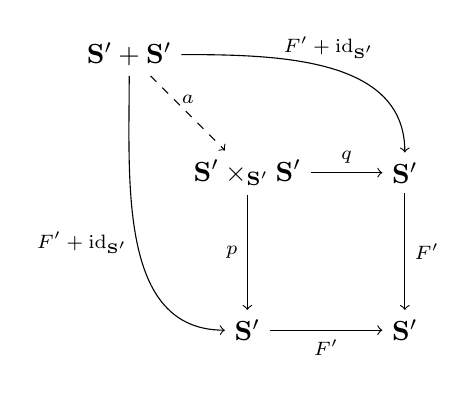
\begin{tikzpicture}
	\node (1) at (-1.5,2.5) {$\cat{S}' + \cat{S}'$};
	\node (2) at (0,1) {$\cat{S}' \times_{\cat{S}'} \cat{S}'$};
	\node (3) at (2,1) {$\cat{S}'$};
	\node (4) at (0,-1) {$\cat{S}'$};
	\node (5) at (2,-1) {$\cat{S}'$};
	%
	\draw [dashed,->] (1) to[] node[above]{\scriptsize $a$} (2);
	\draw [->] (1) to[out=0,in=90] node[above]{\scriptsize $F'+\id_{\cat{S}'}$} (3);
	\draw [->] (1) to[out=-90,in=180] node[left]{\scriptsize $F'+\id_{\cat{S}'}$} (4);
	\draw [->] (2) to[] node[above]{\scriptsize $q$} (3);
	\draw [->] (2) to[] node[left]{\scriptsize $p$} (4);
	\draw [->] (3) to[] node[right]{\scriptsize $F'$} (5);
	\draw [->] (4) to[] node[below]{\scriptsize $F'$} (5);
\end{tikzpicture}
\]
One can check that $a = \Delta (F' + \id_{\cat{S}'})$.

Now, our goal is to show that the span of spans 
\[
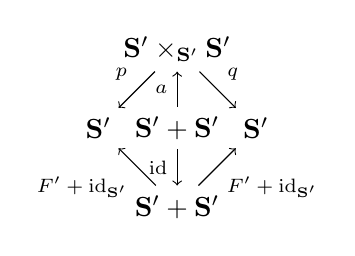
\begin{tikzpicture}
	\node (lleg) at (-1,0) {$\cat{S}'$};
	\node (uapex) at (0,1) {$\cat{S}'\times_{\cat{S}'}\cat{S}'$};
	\node (lapex) at (0,-1) {$\cat{S}'+\cat{S}'$};
	\node (rleg) at (1,0) {$\cat{S}'$};
	\node (mid) at (0,0) {$\cat{S}'+\cat{S}'$};
	%
	\draw [->] (uapex) to node[above left] {\scriptsize $p$} (lleg);
	\draw [->] (uapex) to node[above right] {\scriptsize $q$} (rleg);
	\draw [->] (lapex) to node[below left] {\scriptsize $F'+\id_{\cat{S}'}$} (lleg);
	\draw [->] (lapex) to node[below right] {\scriptsize $F'+\id_{\cat{S}'}$} (rleg);
	\draw [<-] (uapex) to node[left] {\scriptsize $a$} (mid);
	\draw [<-] (lapex) to node[left] {\scriptsize $\id$} (mid);
\end{tikzpicture}
\]
has a weak inverse
\[
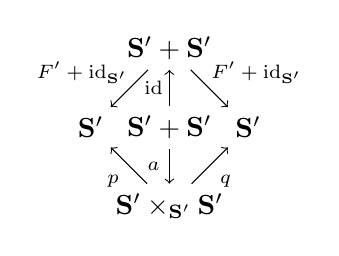
\begin{tikzpicture}
	\node (lleg) at (-1,0) {$\cat{S}'$};
	\node (lapex) at (0,-1) {$\cat{S}'\times_{\cat{S}'}\cat{S}'$};
	\node (uapex) at (0,1) {$\cat{S}'+\cat{S}'$};
	\node (rleg) at (1,0) {$\cat{S}'$};
	\node (mid) at (0,0) {$\cat{S}'+\cat{S}'$};
	%
	\draw [->] (lapex) to node[shift={(-0.2,-0.2)}] {\scriptsize $p$} (lleg);
	\draw [->] (lapex) to node[shift={(0.2,-0.2)}] {\scriptsize $q$} (rleg);
	\draw [->] (uapex) to node[shift={(-0.6,0.2)}] {\scriptsize $F'+\id_{\cat{S}'}$} (lleg);
	\draw [->] (uapex) to node[shift={(0.6,0.2)}] {\scriptsize $F'+\id_{\cat{S}'}$} (rleg);
	\draw [<-] (lapex) to node[shift={(-0.2,0)}] {\scriptsize $a$} (mid);
	\draw [<-] (uapex) to node[shift={(-0.2,0)}] {\scriptsize $\id$} (mid);
\end{tikzpicture}
\]
in the sense that the two possible vertical composites of these are identified with the identity $2$-cells 
\[
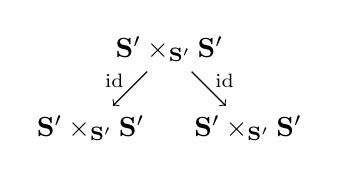
\begin{tikzpicture}
	\node (v1) at (0,2) {$\cat{S'} \times_{\cat{S'}} \cat{S'}$};
	\node (v2) at (-1,1) {$\cat{S'} \times_{\cat{S'}} \cat{S'}$};
	\node (v3) at (1,1) {$\cat{S'} \times_{\cat{S'}} \cat{S'}$};
	\draw [->] (v1) to node[shift={(-0.2,0.1)}] {\scriptsize $\id$} (v2);
	\draw [->] (v1) to node[shift={(0.2,0.1)}] {\scriptsize $\id$} (v3);
\end{tikzpicture}
%
\quad \quad \quad
%
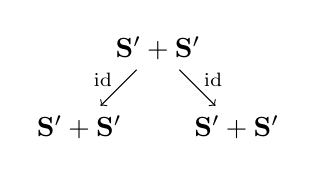
\begin{tikzpicture}
	\node (v1) at (0,2) {$\cat{S'} + \cat{S'}$};
	\node (v2) at (-1,1) {$\cat{S'} + \cat{S'}$};
	\node (v3) at (1,1) {$\cat{S'} + \cat{S'}$};
	\draw [->] (v1) to node[shift={(-0.2,0.1)}] {\scriptsize $\id$} (v2);
	\draw [->] (v1) to node[shift={(0.2,0.1)}] {\scriptsize $\id$} (v3);
\end{tikzpicture}
\]

First, we will calculate the composite
\[
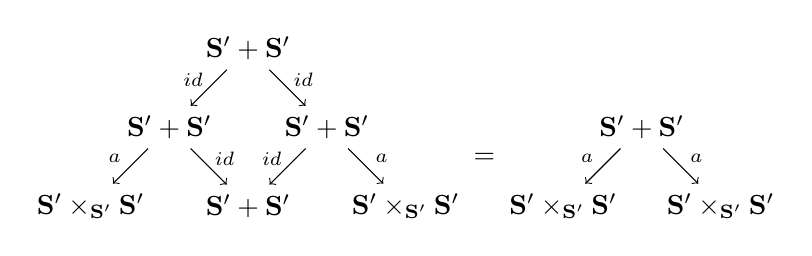
\begin{tikzpicture}
	\begin{scope}
	\node (v1) at (0,2) {$\cat{S}'+ \cat{S}'$};
	\node (v2) at (-1,1) {$\cat{S}' \times_{\cat{S}'} \cat{S}'$};
	\node (v3) at (1,1) {$\cat{S}'+ \cat{S}'$};
	\node (v4) at (2,2) {$\cat{S}'+ \cat{S}'$};
	\node (v5) at (3,1) {$\cat{S}' \times_{\cat{S}'} \cat{S}'$};
	\node (v6) at (1,3) {$\cat{S}'+ \cat{S}'$};
	\draw [->] (v1) to node[shift={(-0.2,0.1)}] {\scriptsize $a$} (v2);
	\draw [->] (v1) to node[shift={(0.2,0.1)}] {\scriptsize $id$} (v3);
	\draw [->]  (v4) edge node[shift={(-0.2,0.1)}] {\scriptsize $id$} (v3);
	\draw [->] (v4) edge node[shift={(0.2,0.1)}] {\scriptsize $a$} (v5);
	\draw [->]  (v6) edge node[shift={(-0.2,0.1)}] {\scriptsize $id$} (v1);
	\draw [->] (v6) edge node[shift={(0.2,0.1)}] {\scriptsize $id$} (v4);
	\end{scope}
	%
	\begin{scope}[shift={(6,0)}]
	\node (v1) at (0,2) {$\cat{S}'+ \cat{S}'$};
	\node (v2) at (-1,1) {$\cat{S}' \times_{\cat{S}'} \cat{S}'$};
	\node (v3) at (1,1) {$\cat{S}' \times_{\cat{S}'} \cat{S}'$};
	\draw [->] (v1) to node [shift={(-0.2,0.1)}] {\scriptsize $a$} (v2);
	\draw [->] (v1) to node [shift={(0.2,0.1)}] {\scriptsize $a$} (v3);
	\end{scope}
	\node at (4,1.6) {$=$};
\end{tikzpicture}
\]



First we obtain the composite 
\[
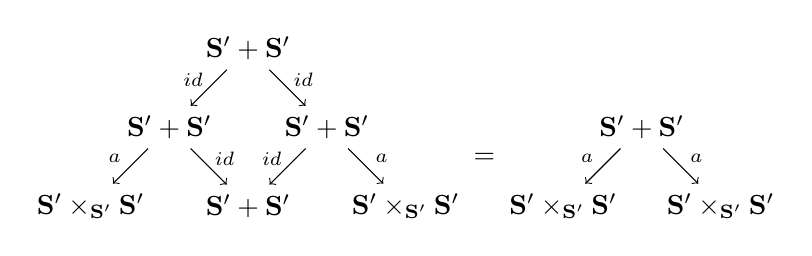
\begin{tikzpicture}
	\begin{scope}
	\node (v1) at (0,2) {$\cat{S}'+ \cat{S}'$};
	\node (v2) at (-1,1) {$\cat{S}' \times_{\cat{S}'} \cat{S}'$};
	\node (v3) at (1,1) {$\cat{S}'+ \cat{S}'$};
	\node (v4) at (2,2) {$\cat{S}'+ \cat{S}'$};
	\node (v5) at (3,1) {$\cat{S}' \times_{\cat{S}'} \cat{S}'$};
	\node (v6) at (1,3) {$\cat{S}'+ \cat{S}'$};
	\draw [->] (v1) to node[shift={(-0.2,0.1)}] {\scriptsize $a$} (v2);
	\draw [->] (v1) to node[shift={(0.2,0.1)}] {\scriptsize $id$} (v3);
	\draw [->]  (v4) edge node[shift={(-0.2,0.1)}] {\scriptsize $id$} (v3);
	\draw [->] (v4) edge node[shift={(0.2,0.1)}] {\scriptsize $a$} (v5);
	\draw [->]  (v6) edge node[shift={(-0.2,0.1)}] {\scriptsize $id$} (v1);
	\draw [->] (v6) edge node[shift={(0.2,0.1)}] {\scriptsize $id$} (v4);
	\end{scope}
	%
	\begin{scope}[shift={(6,0)}]
	\node (v1) at (0,2) {$\cat{S}'+ \cat{S}'$};
	\node (v2) at (-1,1) {$\cat{S}' \times_{\cat{S}'} \cat{S}'$};
	\node (v3) at (1,1) {$\cat{S}' \times_{\cat{S}'} \cat{S}'$};
	\draw [->] (v1) to node [shift={(-0.2,0.1)}] {\scriptsize $a$} (v2);
	\draw [->] (v1) to node [shift={(0.2,0.1)}] {\scriptsize $a$} (v3);
	\end{scope}
	\node at (4,1.6) {$=$};
\end{tikzpicture}
\]
Now, clearly we have a diagram 
\[
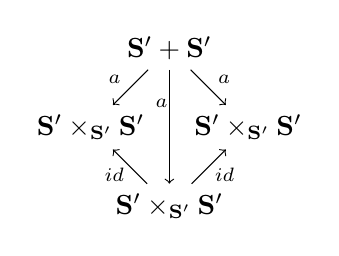
\begin{tikzpicture}
	\node (v1) at (0,2) {$\cat{S}'+ \cat{S}'$};
	\node (v2) at (-1,1) {$\cat{S}' \times_{\cat{S}'} \cat{S}'$};
	\node (v3) at (1,1) {$\cat{S}' \times_{\cat{S}'} \cat{S}'$};
	\node (v4) at (0,0) {$\cat{S}' \times_{\cat{S}'} \cat{S}'$};
	\draw [->] (v1) to node [shift={(-0.2,0.1)}] {\scriptsize $a$} (v2);
	\draw [->] (v1) to node [shift={(0.2,0.1)}] {\scriptsize $a$} (v3);
	\draw [->]  (v4) edge node [shift={(-0.2,-0.1)}] {\scriptsize $id$} (v2);
	\draw [->]  (v4) edge node [shift={(0.2,-0.1)}] {\scriptsize $id$} (v3);
	\draw [->]  (v1) edge node [shift={(-0.1,0.3)}] {\scriptsize $a$} (v4);
\end{tikzpicture}
\]
relating the composite span with the identity span.  Moreover, it commutes exactly. It remains to show that $a$ is an equivalence of groupoids.  However, this is not possible.   

%%%%%%%%%%%%%%%%%%%%%%%%%%%%%%%%%%%%%%%%%%%%%%%%%%%%%%%%%
%%%%%%%%%%%%%%%%%%%%%%%%%%%%%%%%%%%%%%%%%%%%%%%%%%%%%%%%%
%%%%%%%%%%%%%%%%%%%%%%%%%%%%%%%%%%%%%%%%%%%%%%%%%%%%%%%%%
%%%%%%%%%%%%%%%%%%%%%%%%%%%%%%%%%%%%%%%%%%%%%%%%%%%%%%%%%
%
%                                        END DOCUMENT
%
%%%%%%%%%%%%%%%%%%%%%%%%%%%%%%%%%%%%%%%%%%%%%%%%%%%%%%%%%
%%%%%%%%%%%%%%%%%%%%%%%%%%%%%%%%%%%%%%%%%%%%%%%%%%%%%%%%%
%%%%%%%%%%%%%%%%%%%%%%%%%%%%%%%%%%%%%%%%%%%%%%%%%%%%%%%%%
%%%%%%%%%%%%%%%%%%%%%%%%%%%%%%%%%%%%%%%%%%%%%%%%%%%%%%%%%

\end{document}
